%! Licence = CC BY-NC-SA 4.0

%! Author = gianfluetsch
%! Date = 30. Dez 2021
%! Project = cydef_summary

\section{Active Directory}
\begin{itemize}
    \item Active Directory (AD) is a directory service (database) developed by Microsoft
    \item Used for centralized management of computers, servers, users, …
    \item Performs authentication and authorization of users and computers
    \begin{itemize}
        \item It verifies the credentials of the users and defines their access rights
        \item It is based on LDAP, NTLM, Kerberos (Microsoft's version), DNS and other protocols
    \end{itemize}
    \item Structured in objects
    \begin{itemize}
        \item Resources (e.g. printers)
        \item Security Principals (e.g. users, groups, computer accounts)
    \end{itemize}
    \item Organizational Units
    \begin{itemize}
        \item Objects within a domain can be grouped into OUs
        \item OUs can provide a hierarchy to a domain. This simplifies administration
    \end{itemize}
    \item Logical divisions: forest, tree \& domain
    \item Active Directory stores
    \begin{itemize}
        \item password hash of every user
        \item computer hash of every computer
        \color{red}
        \item \textbf{Target for attackers!!!}
    \end{itemize}
\end{itemize}

\subsection{Active Directory Threats}
\begin{itemize}
    \item The AD is a central target for attackers, because if compromised, everything is compromised
    \item AD infrastructure can be very complex and therefore hard to configure and maintain securely
    \item \textbf{Common misconfigurations and pitfalls} that can be abused by attackers:
    \begin{itemize}
        \item No segregation of \textbf{privileged access}, e.g. highly privileged admins interactively log on clients/servers
        \item Service (or User) Accounts with \textbf{weak passwords and SPN (Service Principal Name) set}, even worse if ownership is lost
        \item \textbf{Weak passwords} in general
        \item \textbf{Same local admin password} on all computers
        \item \textbf{Password re-use} in general
        \item \textbf{Credentials on shares} (e.g. Logon Scripts on SYSVOL) where Everyone has read/write access
        \item \textbf{Lack of least-privilege} principle in general
    \end{itemize}
\end{itemize}


\subsection{Logging}
Über eine GPO kann ein Logging-Agent (z.B. der Wazuh-Agent) einfach auf allen gewünschten Servern installiert und konfiguriert werden.
Diesen Agent sollte man so konfigurieren, dass er alle wichtigen und relevanten Logs (z.B. die RDP Logs) ebenfalls an Wazuh weiterleitet.
Danach sind diese Logs auch innerhalb von Wazuh zentral ersichtlich und filterbar.

Dabei werden die Events aus dem EventLog an Wazu weitergeleitet und es kann somit auch nach der \textit{EventID} gefiltert werden.

\subsubsection{EventID 1149}
Successful network authentication (successfully executed an RDP network connection).

Event 1149 is logged when there is a successful RDP logon to the computer. Before Windows 7 and Windows Server 2012, 1149 would be logged for any initiation of an RDP connection, so it was not a useful indicator for an actual successful application of user credentials.

But, that has changed, and all modern OS versions will only log 1149 if the username in the event was successfully authenticated. It also includes the IP address of the source of the connection, which is useful information. If an account is used and successfully authenticates but does not have
permission to RDP to the computer due to other restrictions, event 1149 is not generated.

\newpage

\subsubsection{Phases of RDP-Connection}

\begin{minipage}{0.45\linewidth}
    \begin{enumerate}
        \item Connection Initiation
        \item Basic Settings Exchange
        \item Channel Connection
        \item RDP Security Commencement
        \item Secure Settings Exchange
        \item Optional Connect-Time Auto-Detection
        \item Licensing
        \item Optional Multitransport Bootstrapping
        \item Capabilities Exchange
        \item Connection Finalization
    \end{enumerate}
\end{minipage}
\begin{minipage}{0.5\linewidth}
    \begin{center}
        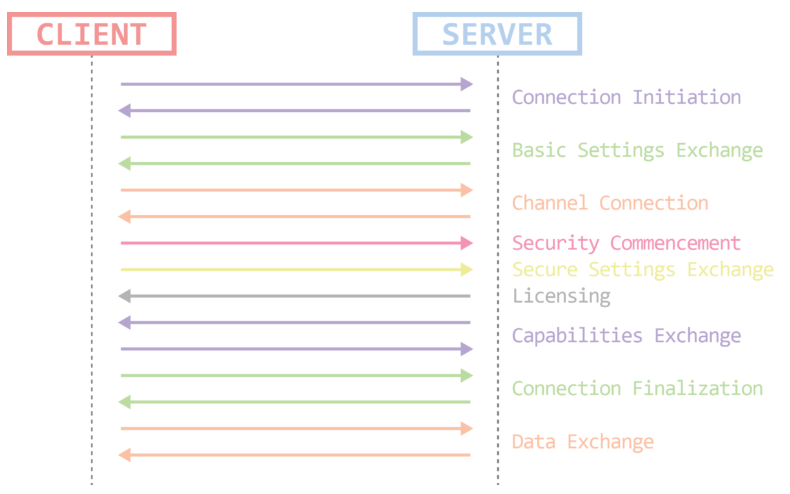
\includegraphics[width=1.2\linewidth]{rdp_phases}
        \vspace{-8pt}
    \end{center}
\end{minipage}

\subsubsection{Explain how you filtered every RDP login attempt}
The TerminalServices-RemoteConnectionManager Log is not forwarded to Wazuh.\\
Unable to filter for all the attempts.
With the current Wazu setup, one must filter for Logon Type 3 \& 10 (remote logon types)\\

\begin{itemize}
    \item \lstinline|data.win.system.eventID = 4624| or \lstinline|data.win.system.eventID = 4625|
    \item \lstinline|data.win.sytem.eventID: 4624| and \lstinline|data.win.evendata.logonType: 3|
\end{itemize}

\subsubsection{Explain how you filtered unsuccessful RDP login attempts}
Um erfolglose RDP Login Versuche im Event Viewer zu suchen, sucht man nach der \lstinline|Event ID: 4625|.\\

\begin{itemize}
    \item \lstinline|data.win.eventdata.logonType = 3| or \lstinline|data.win.eventdata.logonType = 10|
    \item \lstinline|data.win.system.eventID = 4625| and \lstinline|data.win.eventdata.logonType = 3|
\end{itemize}

\subsection{Kerberos}
\begin{minipage}{0.45\linewidth}
    \begin{enumerate}
        \item Client $\rightarrow$ TGS (Ticket Granting Server = DC): \textit{Anfrage}
        \item TGS $\rightarrow$ Client: \textit{TGT (Ticket Granting Ticket)}
        \item Client $\rightarrow$ Fileserver (FS): \textit{TGT}
        \item FS $\rightarrow$ Client: \textit{schön und gut, will aber spezifisches Ticket}
        \item Client $\rightarrow$ TGS: \textit{Anfrage spezifisches Ticket für FS}
        \item TGS $\rightarrow$ Client: \textit{(spezifisches) Ticket für FS}
        \item Client $\rightarrow$ FS: \textit{(spezifisches) Ticket für FS}
        \item FS $\rightarrow$ Client: \textit{alles ok}
    \end{enumerate}
\end{minipage}
\begin{minipage}{0.5\linewidth}
    \begin{center}
        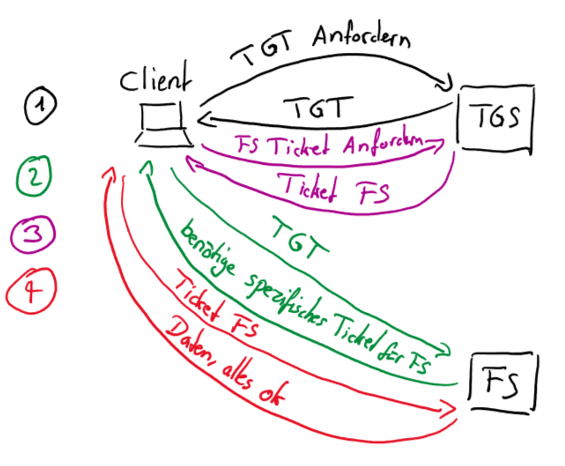
\includegraphics[width=0.9\linewidth]{kerberos}
        \vspace{-8pt}
    \end{center}
\end{minipage}



